\documentclass{mp}
\usepackage[linesnumbered]{algorithm2e}
\DontPrintSemicolon
\graphicspath{{15_prng}}
\subtitle{Generatory liczb pseudolosowych}
\usepackage{listings}


\usepackage{lstlinebgrd} % see http://www.ctan.org/pkg/lstaddons

%http://tex.stackexchange.com/questions/8851/how-can-i-highlight-some-lines-from-source-code
\makeatletter
%%%%%%%%%%%%%%%%%%%%%%%%%%%%%%%%%%%%%%%%%%%%%%%%%%%%%%%%%%%%%%%%%%%%%%%%%%%%%%
%
% \btIfInRange{number}{range list}{TRUE}{FALSE}
%
% Test in int number <number> is element of a (comma separated) list of ranges
% (such as: {1,3-5,7,10-12,14}) and processes <TRUE> or <FALSE> respectively

\newcount\bt@rangea
\newcount\bt@rangeb

\newcommand\btIfInRange[2]{%
    \global\let\bt@inrange\@secondoftwo%
    \edef\bt@rangelist{#2}%
    \foreach \range in \bt@rangelist {%
        \afterassignment\bt@getrangeb%
        \bt@rangea=0\range\relax%
        \pgfmathtruncatemacro\result{ ( #1 >= \bt@rangea) && (#1 <= \bt@rangeb) }%
        \ifnum\result=1\relax%
            \breakforeach%
            \global\let\bt@inrange\@firstoftwo%
        \fi%
    }%
    \bt@inrange%
}
\newcommand\bt@getrangeb{%
    \@ifnextchar\relax%
        {\bt@rangeb=\bt@rangea}%
        {\@getrangeb}%
}
\def\@getrangeb-#1\relax{%
    \ifx\relax#1\relax%
        \bt@rangeb=100000%   \maxdimen is too large for pgfmath
    \else%
        \bt@rangeb=#1\relax%
    \fi%
}

%%%%%%%%%%%%%%%%%%%%%%%%%%%%%%%%%%%%%%%%%%%%%%%%%%%%%%%%%%%%%%%%%%%%%%%%%%%%%%
%
% \btLstHL<overlay spec>{range list}
%
% TODO BUG: \btLstHL commands can not yet be accumulated if more than one overlay spec match.
% 
\newcommand<>{\btLstHL}[1]{%
  \only#2{\btIfInRange{\value{lstnumber}}{#1}{\color{color4!30}\def\lst@linebgrdcmd{\color@block}}{\def\lst@linebgrdcmd####1####2####3{}}}%
}%
\makeatother



\begin{document}
\frame{\titlepage}
\begin{frame}{9}
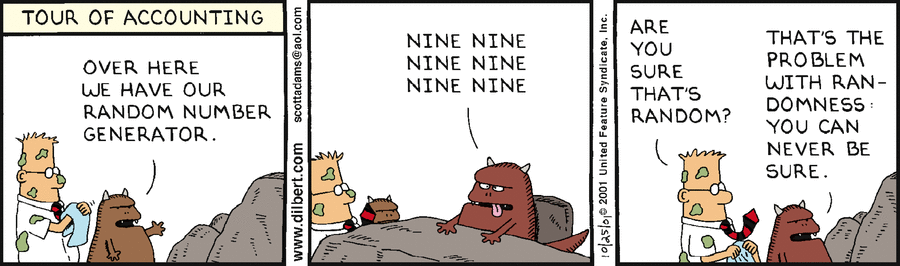
\includegraphics[width=\textwidth]{15_prng/dilbert.png}
\vfill
{\small \url{http://dilbert.com/strip/2001-10-25}}
\end{frame}
\begin{frame}{Ciąg liczb losowych}
\[ (X_1, X_2, \ldots) \]
\pause
\begin{enumerate}
\item $X_i$ mają identyczne rozkłady
\item $X_i$ są niezależne
\end{enumerate}
\end{frame}
\begin{frame}{Generowanie liczb o zadanym rozkładzie}
\begin{description}
\item[wejście] $X\sim\mathcal{U}(0,1)$
\item[wyjście] $Y$ z zadanego rozkładu
\end{description}
\pause
\[ Y=F^{-1}(X) \]
\pause
\[Y\sim Exp(0{,}5) \qquad x=0{,}1563 \]
\note<1>{\[F(y)=1-e^{-\lambda y} \qquad y=
\frac{\ln(1-F(y)}{-\lambda}=
\frac{\ln(1-0{,}1563}{-0{,5}}\approx 0{,}34\]}
\end{frame}
\begin{frame}{A jeżeli odwrotność $F$ nie jest znana?}
\begin{minipage}{.49\textwidth}
\begin{algorithm}[H]
\Repeat{$b-a\leq \delta$}
{
$y\leftarrow \frac{a+b}{2}$ \;
\lIf{$F(y)\leq X$}{$a\leftarrow y$}
\lElse{$b\leftarrow y$}
}
\Return{$y$}
\end{algorithm}
\end{minipage}
\begin{minipage}{.49\textwidth}
\pause
$Y\sim\mathcal{N}(0,1) \qquad x=0{,}1563$ \\
\pause
\begin{tabular}{rrrr}
	$a$	& $b$	& $y$ &	$F(y)$ \\
	\hline
$-10{,}000$	& $10{,}000$ &	$ 0{,}000$ & $0{,}500$ \\
\pause
$-10{,}000$	& \alert{$ 0{,}000$} &	$-5{,}000$ & $0{,}000$ \\
\alert{$ -5{,}000$}	& $ 0{,}000$ &	$-2{,}500$ & $0{,}006$ \\
\alert{$ -2{,}500$}	& $ 0{,}000$ &	$-1{,}250$ & $0{,}106$ \\
\alert{$ -1{,}250$}	& $ 0{,}000$ &	$-0{,}625$ & $0{,}266$ \\
$ -1{,}250$	& \alert{$-0{,}625$} &	$-0{,}938$ & $0{,}174$ \\
$ -1{,}250$	& \alert{$-0{,}938$} &	$-1{,}094$ & $0{,}137$ \\
\alert{$ -1{,}094$}	& $-0{,}938$ &	$-1{,}016$ & $0{,}155$ \\
\alert{$ -1{,}016$}	& $-0{,}938$ &	$-0{,}977$ & $0{,}164$ \\
$ -1{,}016$	& \alert{$-0{,}977$} &	$-0{,}996$ & $0{,}160$ \\
$ -1{,}016$	& \alert{$-0{,}996$} &	$-1{,}006$ & $0{,}157$ \\
$ -1{,}016$	& \alert{$-1{,}006$} &	$-1{,}011$ & $0{,}156$ \\
\alert{$ -1{,}011$}	& $-1{,}006$ &	$-1{,}008$ & $0{,}157$ \\
\end{tabular}
\end{minipage}
\end{frame}
\begin{frame}{A dla rozkładów dyskretnych?}
\begin{minipage}{.49\textwidth}
\begin{algorithm}[H]
$i\leftarrow 1$\;
$s\leftarrow p_1$ \;
\While{$s< X$}
{
$i \leftarrow i+1$\;
$s \leftarrow s+p_i$\;
}
\Return{$y_i$}
\end{algorithm}
\end{minipage}
\pause
\begin{minipage}{.49\textwidth}
$Y\sim \mathcal{B}(30,0{,}3) \qquad x=0{,}1563$ \\
\pause
\begin{tabular}{rrr}
$i=y$ &	$p_i$	& $s$ \\
$1$ & $0{,}000$ & $0{,}000$ \\
\pause
$2$ & $0{,}002$ & $0{,}002$ \\
$3$ & $0{,}007$ & $0{,}009$ \\
$4$ & $0{,}021$ & $0{,}030$ \\
$5$ & $0{,}046$ & $0{,}077$ \\
$6$ & $0{,}083$ & \alert{$0{,}160$} \\
\end{tabular}
\end{minipage}
\end{frame}

\begin{frame}[fragile]{Przypadek szczególny: skrócony rozkład równomierny}
\begin{description}
\item[wejście] $X\sim\mathcal{U}(0,n)$
\item[wyjście] $Y\sim\mathcal{U}(0,m)$
\end{description}
\pause
\begin{lstlisting}[language=Java,linebackgroundcolor={\btLstHL{3}}]
r = new Random(1);
for(int i=0;i<200000*11;i++)
    tab[i] = r.nextInt() % 11;
\end{lstlisting}
\pause
\begin{center}
\includegraphics[width=.6\textwidth]{15_prng/lcg_mod_11_hist.pdf}
\end{center}
\end{frame}
\begin{frame}[fragile]{Przypadek szczególny: skrócony rozkład równomierny}
\begin{lstlisting}[language=Java,linebackgroundcolor={\btLstHL{3}}]
r = new Random(1);
for(int i=0;i<200000*11;) {
    tab[i] = r.nextInt() & 0b1111;
    if(tab[i]<11) i++;
}
\end{lstlisting}
\pause
\vspace{-8mm}
\begin{center}
\includegraphics[width=.7\textwidth]{15_prng/lcg_mod_11_cut_hist.pdf}
\end{center}
\end{frame}
\begin{frame}{To samo z bliska}
\centering
\includegraphics[width=\textwidth]{15_prng/lcg_mod_11_comp.pdf}
\end{frame}
\begin{frame}{Analiza algorytmu}
\begin{description}
\item[wejście] $X_i\sim\mathcal{U}(0,2^n-1)\quad X_i$ niezależne
\item[wyjście] $(Y_1, Y_2, \ldots, Y_l)$\qquad $Y_j\sim\mathcal{U}(0,k-1)\quad 2^{n-1}<k\leq 2^n-1$
\end{description}
\pause
\alert{Ile potrzebujemy liczb na wejściu, żeby wygenerować $l$ liczb na wyjściu?}
\note<2>
{
\tiny
Żeby wygenerować jedną liczbę potrzebujemy $N$ liczb z wejścia, gdzie $N$ ma rozkład geometryczny (pobieramy $X$y do pierwszego sukcesu) z $p=\frac{k}{2^n}$.
Żeby wygenerować $l$ takich liczb, musimy zsumować $l$ zmiennych o takim rozkładzie: $W=N_1+N_2+\ldots+N_l$.
Te zmienne są niezależne, ponieważ $X$y są niezależne.
$EN_i=\frac{1}{p}=\frac{2^n}{k}$, $D^2N_i=\frac{1}{p^2}-\frac{1}{p}=\frac{2^n(2^n-k)}{k^2}$
Z niezależności $EN=l\frac{2^n}{k}$ i $D^2N=l\frac{2^n(2^n-k)}{k^2}$.
Nierówność Czebyszewa:
\[ P(N-EN\geq \varepsilon) \leq P(\left|N-EN\right|\geq \varepsilon)\leq \frac{D^2N}{\varepsilon^2} \]
Niech $\varepsilon=l\varrho$ i $k=2^{n-1}$ (najgorszy możliwy przypadek):
\[ P(N-EN\geq \varepsilon) = P(N\geq l(\frac{2^n}{k}+\varrho)) = P(N\geq l(2+\varrho)) \leq \frac{l2^n2^{n-1}}{2^{2(n-1)}l^2\varrho^2}=\frac{2}{l\varrho^2}  \]
Niech $\varrho=8$ i wtedy $P(N\geq 10l)\leq \frac{1}{32l}$
}
\end{frame}
\begin{frame}{Ciąg liczb losowych}
\[ (X_1, X_2, \ldots) \]
\begin{enumerate}
\item \alert{$X_i\sim\mathcal{U}(0,n)$}  lub \alert{$X_i\sim\mathcal{U}(0,1)$}
\item $X_i$ są niezależne
\end{enumerate}
\end{frame}
\begin{frame}{Linear Congruential Generator (LCG)}
\begin{align*}
X_0 = & \text{seed} \\
X_{n+1} = & (aX_n+c) \mod m
\end{align*}
\end{frame}
\begin{frame}{Równomierność}
\centering
\only<1>{\includegraphics[width=.9\textwidth]{15_prng/lcg_1229_1_2048_hist.pdf}}
\only<2>{\includegraphics[width=.9\textwidth]{15_prng/lcg_65538_2_5040_hist.pdf}}
\only<3>
{
\begin{enumerate}
\item 247, 460, 93, 1658, 1971, 1624, 1145, 230, 47, 420, 85, 18, 1643, 1968, 2033, 2046, 1639, 1148, 1869
\item 362, 1478, 1406, 110, 1982, 398, 2126, 2990, 3422, 1118, 5006, 4430, 4142, 3998, \alert{1406, 110, 1982, 398, 2126}
\end{enumerate}
}
\end{frame}
\begin{frame}{Zasady doboru współczynników}
\begin{block}{Twierdzenie}
LCG ma okres $m$ wtedy i tylko wtedy gdy jednocześnie:
\begin{itemize}
\item $m$ i $c$ są względnie pierwsze,
\item $a-1$ jest podzielne przez wszystkie czynniki pierwsze $m$,
\item $a-1$ jest podzielne przez 4 jeżeli $m$ jest podzielne przez 4.
\end{itemize}
\end{block}
\pause
\begin{minipage}{.49\textwidth}
\includegraphics[width=\textwidth]{15_prng/lcg_1229_1_2048_hist.pdf}
\end{minipage}
\begin{minipage}{.49\textwidth}
\begin{tikzpicture}
    \node[anchor=south west,inner sep=0] (image) at (0,0) {\includegraphics[width=\textwidth]{15_prng/lcg_65538_2_5040_hist.pdf}};
    \begin{scope}[x={(image.south east)},y={(image.north west)}]
    	\draw[color4,very thick] (.05,.05) -- (.95,.95);
    	\draw[color4,very thick] (.05,.95) -- (.95,.05);
	\end{scope}
\end{tikzpicture}
\end{minipage}
\end{frame}

\begin{frame}{Zajrzyjmy do kodu}
\url{grepcode.com/file/repository.grepcode.com/java/root/jdk/openjdk/8u40-b25/java/util/Random.java\#Random.next\%28int\%29}
{
\small
\lstinputlisting[language=Java, firstline=88, lastline=90]{15_prng/Random.java}
\ldots
\lstinputlisting[language=Java, firstline=198, lastline=206]{15_prng/Random.java}
}
\end{frame}

\begin{frame}{Niezależność w LCG}
\begin{block}{Ciąg liczb losowych}
\[ (X_1, X_2, \ldots) \]
\begin{enumerate}
\item $X_i\sim\mathcal{U}(0,n)$  lub $X_i\sim\mathcal{U}(0,1)$
\item \alert{$X_i$ są niezależne}
\end{enumerate}
\end{block}
\[ P(X_{n+1}=7|X_n=7) = \alert{\ldots} \]
\pause
\[ P(X_{n+1}=7 \cup X_{n+2}=7 \cup \ldots \cup X_{n+m-1}=7|X_n=7) = \alert{\ldots} \]
\pause
\[ P(X_{n+m}=7|X_n=7) = \alert{\ldots} \]
\end{frame}


\begin{frame}{Bibliografia}
\begin{enumerate}
\item ,,The Art of Computer Programming'' (Vol. 2) D. Knuth, rozdział III
\item ,,Non-Uniform Random Variate Generation'' L. Devroye \url{http://www.nrbook.com/devroye/}
\end{enumerate}
\end{frame}
\end{document}
